
\documentclass{exam}

\usepackage{fullpage}
\usepackage{enumerate}
\usepackage{siunitx} 
\usepackage{graphicx}
\usepackage[fleqn]{amsmath}
\usepackage{cancel}
\usepackage{polynom}
\usepackage{float}
\usepackage{mdwlist}
\usepackage{booktabs}
\usepackage{cancel}
\usepackage{polynom}
\usepackage{caption}

\newcommand{\degree}{\ensuremath{^\circ}} 
\everymath{\displaystyle}

% \begin{figure}[H]
%   \centering
%   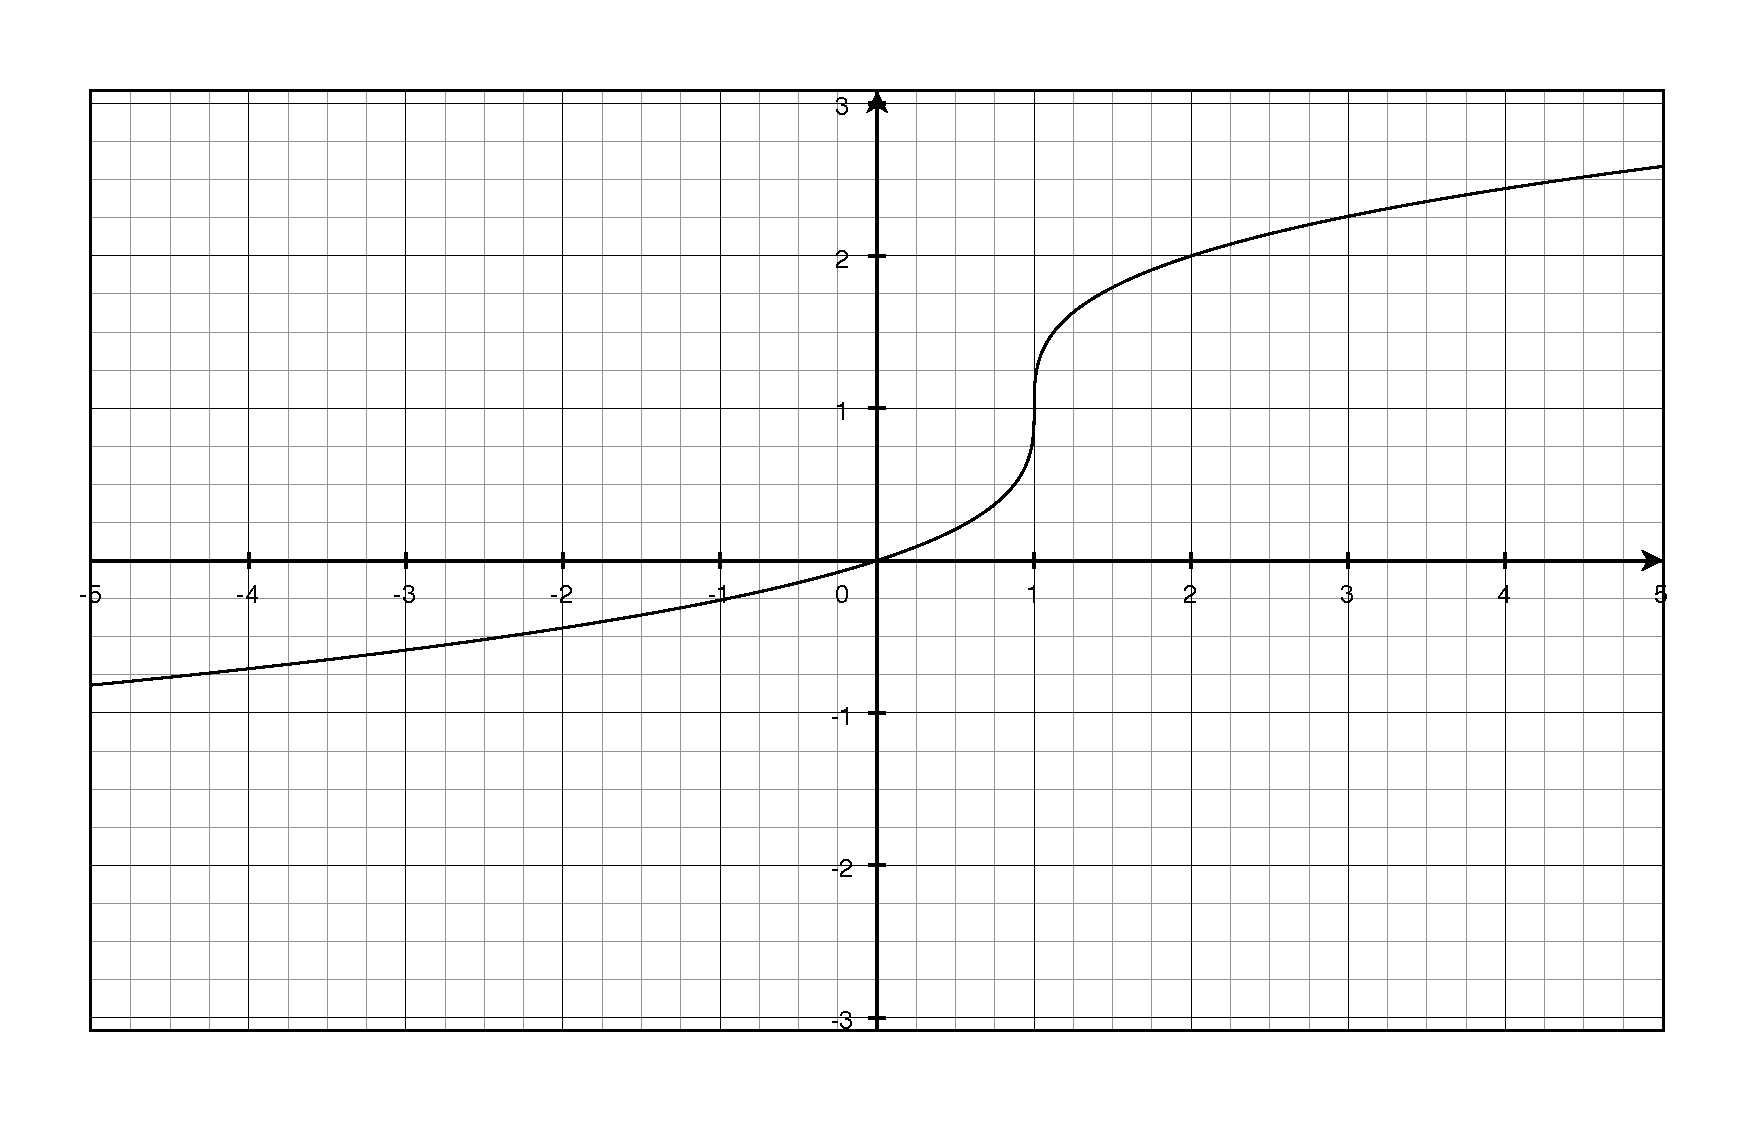
\includegraphics[scale=.3]{question7.eps}
%   \caption*{Question 7}
% \end{figure}

% \begin{tabular}{cc}
% \toprule
% period & amplitude \\
% \midrule
%   $\pi$ & $2$ \\
% \bottomrule
% \end{tabular}

% \textwidth 6.5 in

% \printanswers

\ifprintanswers 
\usepackage{2in1, lscape} 
\fi

\title{Math 263a \\ Practice Problems Week Two}
\date{January 25, 2012}

\begin{document}

\maketitle

\begin{questions}
\question
\begin{align*}
  f(x) &= \frac{1}{x} \\
  g(x) &= \sqrt{x + 2}
\end{align*}

Find the functions and their domains:
\begin{enumerate}[(a)]

\item $(f \cdot g)(x)$
\item $(f \circ g)(x)$
\item $(g \circ f)(x)$
\item $(f \circ f)(x)$
\item $(f/g)(x)$

\end{enumerate}


\question
If $f(x) = \frac{1}{\sqrt[3]{x^2 - 2}}$, find $g$ and $h$ so that $f(x) = (g \circ h)(x)$


\question
Graph $f(x) = \sqrt{x - 1} + 2$

\question
Graph $f(x) = (x + 2)^2 - 3$

\question
Evaluate:
\begin{enumerate}[(a)]
\item $\tan \left( \frac{\pi}{6} \right)$
\item $\sec \left( \frac{\pi}{4} \right)$
\item $\tan \left( -\frac{\pi}{4} \right)$
\item $\csc \left( \frac{3\pi}{4} \right)$
\end{enumerate}

\question
Graph $f(x) = 2 \cos(x)$

\question
Graph $f(x) = \cos(2x)$

\question
Verify each identity:
\begin{enumerate}[(a)]

\item $\cos^2 x - \sin^2 x = 1 - 2 \sin^2 x$

\item $\cot x + \tan x = \csc x \sec x$

\item $\sec x - \cos x = \sin x \tan x$

\end{enumerate}
\end{questions}

\end{document}

